\documentclass[12pt]{article}
\usepackage[english]{varioref}
\usepackage{setspace}
\usepackage[margin=2.54cm]{geometry}
\usepackage{pdfpages}
\usepackage[utf8]{inputenc}
\usepackage[english]{babel}
\usepackage{graphicx,subcaption}
\usepackage{graphics}
\usepackage{lscape}
\usepackage{pdflscape}
\usepackage{float}
\usepackage{textcomp}
\usepackage{amsmath}
\usepackage{hyperref}
\usepackage{fancyvrb}
\usepackage{parskip}
\usepackage{changepage}
\usepackage{enumitem}
\usepackage{tcolorbox}
\usepackage[all]{hypcap}
\usepackage{xcolor}
\usepackage{listings}
\definecolor{green}{HTML}{228B22}
\definecolor{orange}{HTML}{FFC107}
\usepackage{color}
\definecolor{dkgreen}{rgb}{0,0.6,0}
\definecolor{gray}{rgb}{0.5,0.5,0.5}
\definecolor{mauve}{rgb}{0.58,0,0.82}
\lstset{escapeinside={<@}{@>}}

\hypersetup{
    colorlinks,
    citecolor=black,
    filecolor=black,
    linkcolor=black,
    urlcolor=black
}


\lstset{frame=tb,
    language=java,
    aboveskip=3mm,
    belowskip=3mm,
    showstringspaces=false,
    columns=flexible,
    basicstyle={\small\ttfamily},
    numbers=none,
    numberstyle=\tiny\color{gray},
    keywordstyle=\color{blue},
    commentstyle=\color{dkgreen},
    stringstyle=\color{mauve},
    breaklines=true,
    breakatwhitespace=true, tabsize=3
}
\title{
	\begin{center}
	\vspace{3cm}
	\includegraphics[width=11cm, height=3cm]{Images/Logo-nou-eps.jpg}
	\end{center}
	\begin{center}
	\line(1,0){340}
	\end{center}		
	DISTRIBUTED COMPUTING\\
	\vspace{2mm}
	\Large Recent advances and new challenges \\
	\line(1,0){340}
	\vspace{2.5cm}
	}

\author{Marc Cervera Rosell - 47980320C \vspace{1cm}}


\date{Academic course 2022 - 2023\vspace{0.5cm} \\Bachelor's degree in computer engineering}
\onehalfspacing

\begin{document}
	\begin{titlepage}
		\maketitle
		\thispagestyle{empty}
	\end{titlepage}
	\cleardoublepage
	\newpage

\tableofcontents
\listoffigures
\thispagestyle{empty}

\newpage
\section*{Introduction}
\addcontentsline{toc}{section}{Introduction}
On November 23rd, Sergio Trujillo, a BonÀrea worker, came to the distributed computing class to speak about his job in the company.
BonÀrea has a vast experience in the agri-food sector. The company develops all the necessary livestock, industrial and commercial activities to arrive to the consumer with no intermediaries.\\
From 1959, the company has been incorporating in the productive, business and commercial structure all the necessary elements to perform a vertical integration and, in this way, close the complete productive circle of the meat product.
This company, however, has more business lines, such are; animal feeding, agricultural services, energy, finances, insurances, consultant, communications, and supermarkets. Also, has some social actions as BonÀrea foundation assistance and BonÀrea foundation sport.\\
Under the slogan “innovation is our breath”, BonÀrea has always bet on technology and tried to keep it in mind in all the productive cycle. Starting with the digitalization of the primary sector, going through the industrial activities and finally with the distribution of their products. This is possible thanks to a team formed by more than 200 professionals distributed in different areas inside the company.\\
Under the slogan “innovation is our breath”, BonÀrea always has bet on technology and tried to keep it in mind in all the productive cycle. Starting with the digitalization of the primary sector, going through the industrial activities and finally with the distribution of their products. This is possible thanks to a team formed by more than 200 professionals distributed in different areas inside the company.\\
Referring to the technological development, the company has always bet for its own personal, by providing all kinds of formations and giving the chance of having a professional development inside an area where, historically, always has had shortcomings and challenges.\\
The BonÀrea's technological area is segmented in 8 different subareas: App development, Big data, E-commerce, ERP solutions, AI, industry 5.0, cybersecurity and systems.\\
The first computer, arrived to the company in 1969. From then until nowadays, the company developers have written thousands of code lines and the company data centres have processed millions of data and petitions to make all the services have an optimum stability. All of this is achieved analysing and monitoring all the data 24 hours a day, 7 days a week.\\
In the following image, the BonÀrea IT's logo can be seen.
\begin{figure}[H]
    \centering
    
\includegraphics[scale = 0.2]{Images/bonarea-it.jpg}
    \caption{BonÀrea IT's logo}
    \label{fig:ITlogo}
\end{figure}
\pagenumbering{arabic}
\section*{Activity questions}
\addcontentsline{toc}{section}{Activity questions}
\subsection*{Question 1}
\addcontentsline{toc}{subsection}{Question 1}
\textbf{What main technologies do they use and for what purpose do each of them?}
\subsubsection*{Unibasic}
\addcontentsline{toc}{subsubsection}{Unibasic}
UniBasic is an interactive Business BASIC development language that operates on a wide range of Unix-based systems.
This technology is currently used as a database. $\longrightarrow$ BonÀrea uses this techonology for the boxes.\\
The boxes are open-air centres where you can collect your food purchase. There are available fridges and freezers.\\
The biggest disadvantage, it's that Unibasic uses as many licences as open terminals. 
\begin{figure}[H]
    \centering
    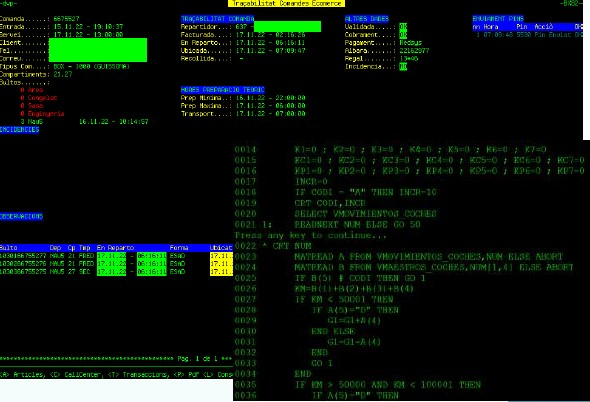
\includegraphics[scale = 0.7]{Images/unibasic.jpg}
    \caption{Example of Unibasic's code}
    \label{fig:unibasic}
\end{figure}
\subsubsection*{Visual Basic}
\addcontentsline{toc}{subsubsection}{Visual Basic}
This is an obsolete technology. The last stable version (Visual Basic 6.0), was released in 1998. $\longrightarrow$ BonÀrea used this technology to perform the interaction between the operating system and the devices.
\begin{figure}[H]
    \centering
    
\includegraphics[scale = 0.7]{Images/VB-6.0.png}
    \caption{Visual Basic's starting layout}
    \label{fig:VB}
\end{figure}
The biggest disadvantages of Visual basic are that the client have to install libraries and software, and uses as many licenses as open terminals.
\subsubsection*{ASP/PHP}
\addcontentsline{toc}{subsubsection}{ASP/PHP}
These two technologies are programming languages that adapt well, specially, to the web developing. The main difference between them is that ASP is property of Microsoft and PHP has a free software license. $\longrightarrow$ BonÀrea used these two technologies to build the webpage in the past.\\
Let's see an example of PHP code:\\
Let's begin with the server side:
\begin{lstlisting}
    <html>
        <head>
            <tittle>PHP Test</tittle>
        </head>
        <body>
            <?php echo '<p>Hello World</p>'; ?>
        </body>
    </html>
\end{lstlisting}
The biggest disadvantage of using this technologies are that each request opens and closes independent connections to the DB and the full page is sent on each query.\\
While it's that using the browser as the terminal provides more security, it's hard to control the external components and devices and there are differences between browsers.
\subsubsection*{jQuery/Bootstrap}
\addcontentsline{toc}{subsubsection}{jQuery/Bootstrap}
With the advent of web 2.0, jQuery was one of the most widely used libraries to facilitate DOM management and make AJAX calls. $\longrightarrow$ BonÀrea used this technology to build the webpage in the past.
\begin{figure}[H]
    \centering
    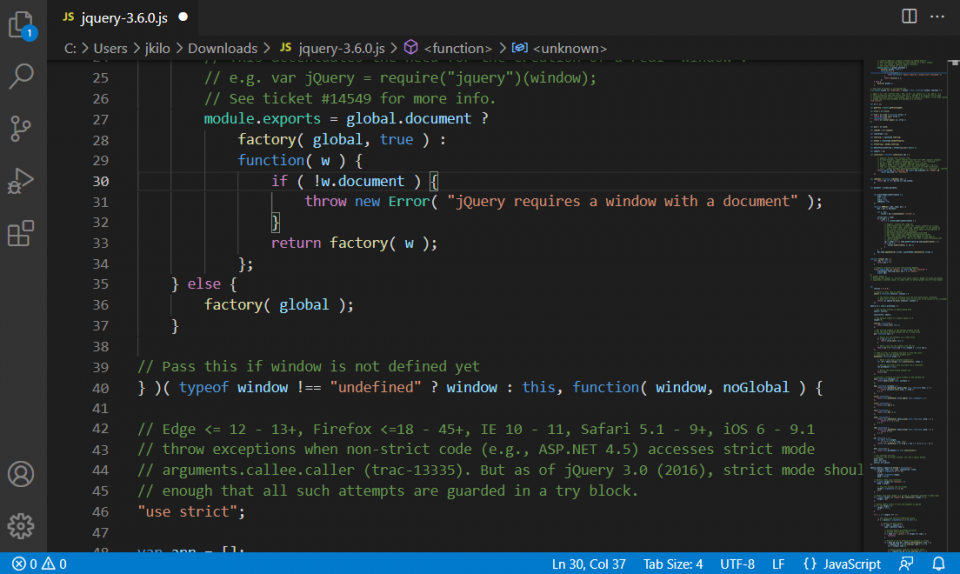
\includegraphics[scale = 0.7]{Images/1639283353HPj4hCHgBW.png}
    \caption{jQuery code example}
    \label{fig:jQuery}
\end{figure}
\subsubsection*{Polymer}
\addcontentsline{toc}{subsubsection}{Polymer}
Polymer is an open-source JavaScript library for web applicastions using web components. $\longrightarrow$ BonÀrea used this technology to built his page. Polymer became obsolete.
\subsubsection*{SPA/PWA}
\addcontentsline{toc}{subsubsection}{SPA/PWA}
PWA is understood as a progressive web app. It is a mobile app in a browser that has gradually become an alternative to native apps. The term PWA was coined originally by Google, which established a checklist to define what creates a PWA. PWA is built from web technologies that are quite similar to us, like HTML, JavaScript, and CSS.\\
SPA stands for a single-page application. It is a web application in which its content is dynamically loaded without reloading the page.\\
In SPA, when you open one page, all HTML and CSS are loaded instantly. Then, when you move around this site, only the updated data is loaded; the page is not necessary to reload. This is the reason why the user experience becomes smoother without wasting time waiting for loading.\\
So, BonÀrea uses these technologies to create his website.
\begin{figure}[H]
    \centering
    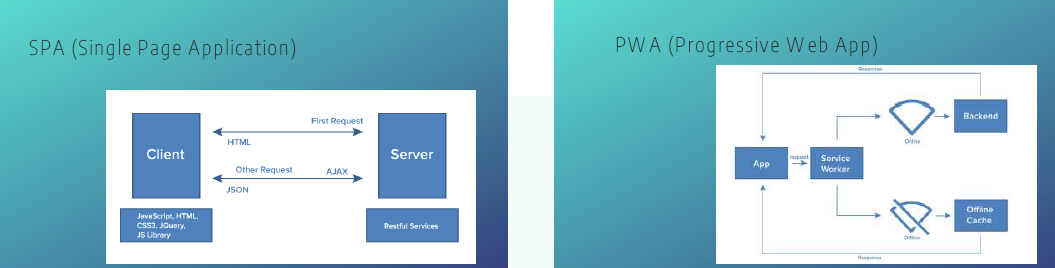
\includegraphics[scale = 0.45]{Images/spa-pwa.png}
    \caption{SPA/PWA schema}
    \label{fig:spa-pwa}
\end{figure}
\subsubsection*{Java/JAKARTAEE}
\addcontentsline{toc}{subsubsection}{Java/JAKARTAEE}
These technologies are used to code all the backend.\\
JakartaEE is the new equivalent of JavaEE. This means that the company has to migrate from JavaEE to JakartaEE. JavaEE (JakartaEE now) provided a lot of tools to work efficiently and in an ordered way.
\begin{figure}[H]
    \centering
    
\includegraphics[scale = 0.7]{Images/jakarta ee-1.jpg}
    \caption{Jakarta's logo}
    \label{fig:jakarta}
\end{figure}
\subsubsection*{Microprofile}
\addcontentsline{toc}{subsubsection}{Microprofile}
This technology is currently used to update dependencies from \textit{javax} to \textit{jakarta}.
\begin{figure}[H]
    \centering
    
\includegraphics[scale = 0.7]{Images/microprofile.jpg}
    \caption{Microprofile's logo}
    \label{fig:microprofile}
\end{figure}
\subsubsection*{Docker/Kubernates}
\addcontentsline{toc}{subsubsection}{Docker/Kubernates}
BonÀrea uses these technologies to create the structure the softwtare structure through code.
\subsubsection*{WAF}
\addcontentsline{toc}{subsubsection}{WAF}
This technology is the most recent implementation speaking of security.
\begin{figure}[H]
    \centering
    
\includegraphics[scale = 0.2]{Images/waf.png}
    \caption{WAF's logo}
    \label{fig:waf}
\end{figure}
\subsubsection*{SOC/SIEM}
\addcontentsline{toc}{subsubsection}{SOC/SIEM}
This technology is used by the company for security issues. Concretely, is used for ensuring the security of the information and reviewing alerts that will detect an attack.\\
\subsubsection*{SQL Server}
\addcontentsline{toc}{subsubsection}{SQL Server}
SQL Server, is used for the data integration to the business intelligence systems.
\begin{figure}[H]
    \centering
    
\includegraphics[scale = 0.3]{Images/sql server.png}
    \caption{SQL server's logo}
    \label{fig:SQL}
\end{figure}
\subsubsection*{MySQL/MariaDB/InfluxDB/MongoDB/Redis/IndexedDB/Universe}
\addcontentsline{toc}{subsubsection}{MySQL/MariaDB/InfluxDB/MongoDB/Redis/IndexedDB/Universe}
All of these technologies are databases.\\
Except MongoDB, the other ones are SQL or SQL-like databases. MongoDB is a non relational database and is used as a support to provide more velocity.\\
Redis is used as a caché. Redis is a key-value DB and the where the "value" values are JSON.\\
InfluxDB is used in the company to manage the the operational technology of the company and is very similar to SQL.\\
Universe is the database that contains approximately the 90\% of the code that the workers codify and have codified all over the years. It's a multivalue database and is used by BonÀre since the 70's.\\
Finally, IndexedDB, is a database that is integrated inside the browsers.
\begin{figure}[H]
    \centering
    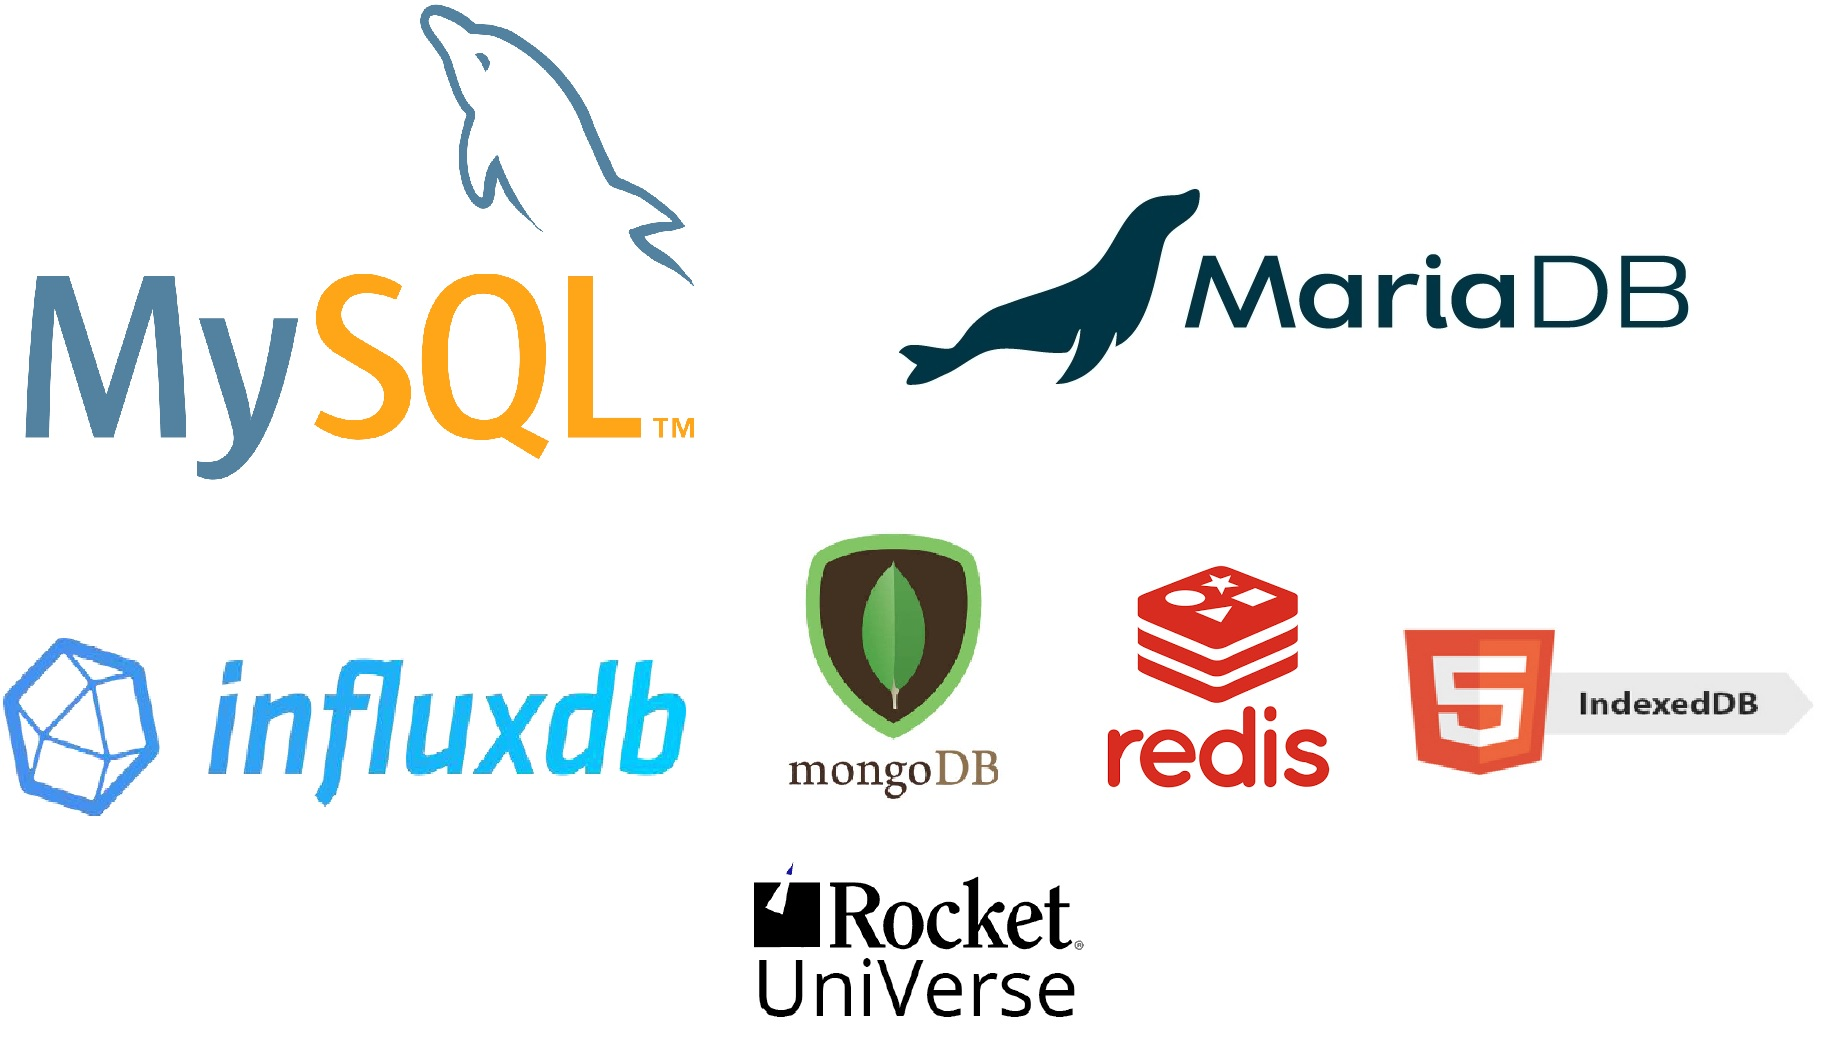
\includegraphics[scale = 0.3]{Images/logos varis.jpg}
    \caption{From left to right and from up to down. Logos of: MySQL, MariaDB, influxDB, mongoDB, redis, indexedDB and universe.}
    \label{fig:dbs}
\end{figure}
\subsubsection*{Elsatic search/apache lucene - apache solar}
\addcontentsline{toc}{subsubsection}{Elsatic search/apache lucene - apache solar}
These technologies are search engines and are used by the company because they provide many options to improve the obtained results.
\begin{figure}[H]
    \centering
    
\includegraphics[scale = 0.7]{Images/apache.jpg}
    \caption{From left to right. Apache lunar and apache solr.}
    \label{fig:apache}
\end{figure}
\subsubsection*{Queues}
\addcontentsline{toc}{subsubsection}{Queues}
Actually, queues are not a technology. Actually are a data-structure that are integrated inside different technologies.
In this section, appear messaging brokers such are RabbitMQ, Kafka and ActiveMQ. These technologies are messagin brokers. So, are intermediary computer programs that translate a message from the formal messaging protocol of the sender to the formal messaging protocol of the receiver.\\
Message brokers are elements in telecommunication or computer networks where software applications communicate by exchanging formally-defined messages.[1] Message brokers are a building block of message-oriented middleware (MOM) but are typically not a replacement for traditional middleware like MOM and remote procedure call (RPC).\\
One thing to highlight of Kafka, is that is less flexible than RabbitMQ but has the advantage that the messages are persistent and we can retrieve them.
\subsubsection*{Saga pattern}
\addcontentsline{toc}{subsubsection}{Saga pattern}
The Saga design pattern is a way to manage data consistency across microservices in distributed transaction scenarios. A saga is a sequence of transactions that updates each service and publishes a message or event to trigger the next transaction step. If a step fails, the saga executes compensating transactions that counteract the preceding transactions.
\begin{figure}[H]
    \centering
    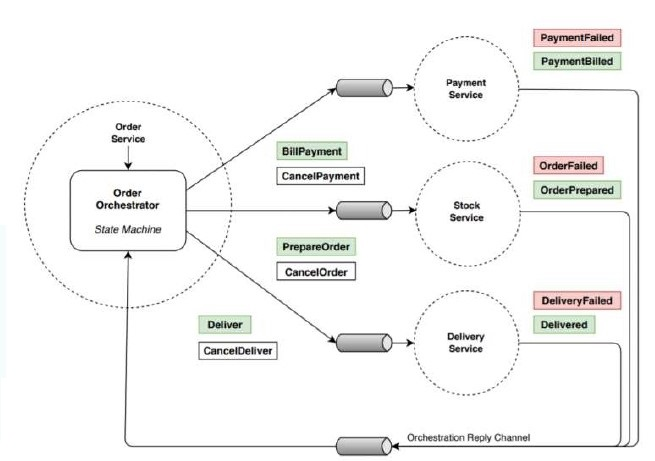
\includegraphics[scale = 0.8]{Images/saga_bo.jpg}
    \caption{Saga pattern according to a BonÀrea's order}
    \label{fig:saga}
\end{figure}
\section*{Question 2}
\addcontentsline{toc}{section}{Question 2}
\textbf{Which criteria have they followed to choose the development technologies? Efficiency, performance, standarizartion, open systems, or does it respond to an integration with old systems?}\\
To answer the second question of this activity, all the technologies will be listed identifying the reason why they were chosen.
\begin{itemize}
    \item Java
    \begin{itemize}
        \item Standard.
        \item Efficient.
        \item Solid. $\longrightarrow$ Has no weaknesses nor security gaps.
    \end{itemize}
    \item Kubernates
    \begin{itemize}
        \item Efficient
        \begin{itemize}
            \item Allow working with multiple dockers.
            \item Allow saving the dockers logs.
            \item And more!
        \end{itemize}
    \end{itemize}
    \item WAF
    \begin{itemize}
        \item Protective shield.
        \item Detect the action of automatted attacks.
        \item App level (layer 7s) control.
    \end{itemize}
    \item Unibasic
    \begin{itemize}
        \item Fast.
        \item Long term.
    \end{itemize}
    \item ASP/PHP
    \begin{itemize}
        \item Easy.
    \end{itemize}
    \newpage
    \item On premise (No cloud)
    \begin{itemize}
        \item Data protection.
        \item Unrestricted access.
        \item Own maintenance.
    \end{itemize}
    \item MariaDB/MySQL
    \begin{itemize}
        \item Replication between instances is very spontaneous.
        \item GNU license.
        \item Fast.
        \item Easy integration with a wide variety of software tools.
    \end{itemize}
    \item SQL server
    \begin{itemize}
        \item Data security.
        \item Frequent/Standard.
    \end{itemize}
    \item InfluxDB
    \begin{itemize}
        \item SQL-like language for queries.
        \item Low latency (nearly real time).
        \item OSS license.
    \end{itemize}
    \item MongoDB
    \begin{itemize}
        \item No schema predefined $\longrightarrow$ Flexibility.
        \item No need extra format conversion.
        \item SSPL license (Almost OSS license).
    \end{itemize}
    \item Redis
    \begin{itemize}
        \item Provides services continuously.
        \item Can withstand failures.
        \item Fast.
        \item Clients can be implemented in all the popular programming languages.
    \end{itemize}
    \item Apache lucene and Apache Solar
    \begin{itemize}
        \item Elastic search.
        \begin{itemize}
            \item Provide many options to improve the obtained results.
        \end{itemize}
    \end{itemize}
    \item Universe
    \begin{itemize}
        \item Provides a user interface (Command line).
        \item Programming in Unibasic.
        \begin{itemize}
            \item In the previous section, it has been explained that the origins of the company are based on this language.
        \end{itemize}
        \item Long term. $\longrightarrow$ The company has a lot of years of experience and self-developed resources.
    \end{itemize}
    \item Queues
    \begin{itemize}
        \item Allow decoupling.
        \item It's fault tolerant.
        \item Allow broadcasting.
        \item Flow control.
        \item Load balancing. $\longrightarrow$ Load balancing is the process of distributing a set of tasks over a set of resources (computing units), with the aim of making their overall processing more efficient. Load balancing can optimize the response time and avoid unevenly overloading some compute nodes while other compute nodes are left idle.
    \end{itemize}
    \item JavaEE/Jakarta
    \begin{itemize}
        \item GNU license.
        \item Is developen un Java, hence, complies with the Java properties.
        \item Simplified architecture.
        \item Freedom of choice in servers, tools, and components.
        \item Integration with existing information systems.
        \item Scalability to meet demand variations.
        \item Flexible security model(J2EE).
    \end{itemize}
\end{itemize}
\section*{Question 3}
\addcontentsline{toc}{section}{Question 3}
\textbf{What software architecture is commonly usded in BonÀrea? (Comment if it's a specific design for each application or if there exist a general architecture design).}\\
The main architecture of the company is the virtual servers. They have +500 virtual machines, +1 petabyte of storage,  +8 terabytes of RAM and +1 petahertz of processing power.
They have an applications' server that follows the following scheme:
\begin{figure}[H]
    \centering
    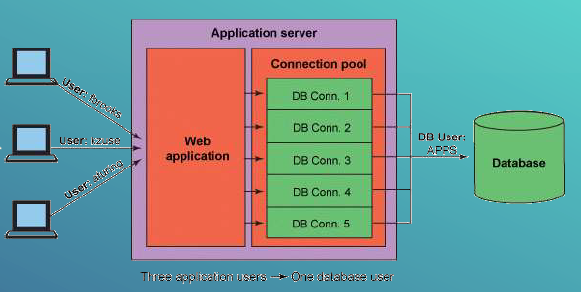
\includegraphics[scale = 0.7]{Images/image_2022-11-28_204332349.png}
    \caption{Apps' server}
    \label{fig:app_server}
\end{figure}
They use Dockers too, to build the structure of a program through code, and finally they use Kubernetes.
\begin{figure}[H]
    \centering
    
\includegraphics[scale = 0.7]{Images/dockerkubernetes.jpg}
    \caption{From left to right: Docker's logo and Kubernetes' logo}
    \label{fig:dockerkubernetes}
\end{figure}
\section*{Question 4}
\addcontentsline{toc}{section}{Question 4}
\textbf{What paradigms of those seen in classroom can you identify that are used on the solutions provided by the lecturer on that company? Discuss about if there has been an evolution or if there are paradigms that have not changed over time.}\\
During the lecture, I was able to identify four different programming paradigms. These paradigms are:
\begin{enumerate}
    \item Message-oriented.
    \item Service-oriented.
    \item Object-oriented.
\end{enumerate}
\section*{Question 5}
\addcontentsline{toc}{section}{Question 5}
\textbf{This company have many different business areas. In most cases it is necessary and important for the company to share these data. How do they solve the sharing of data and/or integration of different applications?}\\
Until 2016 this aspect was not taken in consideration. In 2016 BonÀrea created the "Direcció general". With the creation of this department, the company became centralized, speaking in terms of billing.  A couple of years later, they realized that this was not a perfect system, and they decided to decentralize the company again. But this time, it was not a total decentralization. Nowadays, the company performs a hybrid system in terms of billing.
Now the question is. How can a worker of the company know what is being done in  another department? The answer is easy, a worker can know it through BonÀrea IT.
\section*{Question 6}
\addcontentsline{toc}{section}{Question 6}
\textbf{Regarding the concepts seen in class, how do they address aspects such as availability, accessibility, transparency, openness, scalability, fault tolerance? How do they deal with security aspects?}\\
In terms of security, they use CVE to identify, define and catalog publicly disclosed cybersecurity vulnerabilities. They are forming the users through basic cybersecurity courses. Themselves are sending fishing emails and if the user falls into the trap, the company sends that user to the course.\\
Previously, I've commented about virtual servers. Virtual servers provide a cost reduction, scalability, personalization, easy maintainance and an easy data recovery.\\
In terms of data sharing, they started passing the data with 3+1⁄2-inch floppy disks. Later they changed the system and they were sharing data via telephone. The third data sharing improvement was sharing the data via internet (only 1 time per day) and now, they're sharing data via internet but they're sharing it in real time.\\
BonÀrea is currently renewing the communications ring with a fiber speed of 40 Gb/s x2. In such a way that if one side of the ring goes down, the other side keeps on. It's true, the fact that if one side of the ring goes down, the speed is reduced to 40Gb/s.\\
The network of the company has aproximately 10.000 network ports with 150 subnetworks. $\longrightarrow$ The management of the entire system requires the control and the monitorization of all the resources (VLAN).\\
Using queues, BonÀre achieves concepts as failures tolerance, decoupling, broadcasting, flux control and load balancing.\\
The data sharing among the business areas is performed with web services.
\section*{Question 7}
\addcontentsline{toc}{section}{Question 7}
\textbf{What about the future trends in tools and software development in the company?}\\
The company is focused in target all the technology in web services.
\section*{Conclusions}
\addcontentsline{toc}{section}{Conclusions}
The lecturer claimed that BonÀrea bets for technology, but I don't agree at 100\%. I don't agree because they're using technology that is completely obsolete. Two examples of this are that they are using Unibasic and Rocket Universe.\\
In the other side, they're trying to renew his technologies day to day, but in the BonÀrea's case will cost a couple of years because they have many code to renovate. For example, the lecturer assured that the company used JavaEE but they're now migrating the JavaEE code to Jakarta.
The speaker assured that more than the 90\% of the companie's code is written in Rocket Universe. In my opinion they should do an extra effort to migrate that code to more modern technologies.\\
Apart from my conclusions about the conference, I think that is an interesting activity to know how the company has evolved from his origins to now. \\
It is also interesting to know which technologies were used before those we use today. For example, in my case, I've never listened nothing about Unibasic.\\
\end{document}
